\documentclass{article}

\usepackage[top=20mm, bottom=20mm, left=20mm, right=25mm, 
            marginparwidth=4.5cm, marginparsep=3mm]{geometry}
\usepackage{url}
\usepackage[hidelinks]{hyperref}
%\usepackage[colorlinks=false]{hyperref}
\usepackage{graphicx}
\usepackage{longtable}
\usepackage{subfigure}
\usepackage{parskip}
\usepackage{color}

\newcommand{\henry}{{\bf\Large HENRY}}
\usepackage{xspace}
\newcommand{\defaultServer}{{\url{https://server.psypad.net.au/}\xspace}}
\newcommand{\ImageManagement}{Images\xspace}



\begin{document}

{\Large\centering\bf PsyPad User Manual}

\section*{Introduction}

PsyPad 2.0 has two modes of operation: Demo mode and Participant mode.
Demo mode allows you to run psychophysics experiments (both your own
and the demonstration experiments in the public gallery) and view their
results on the iPad immediately.
Participant mode allows you to configure experiments for participants
where multiple experiments can be presented sequentially with the
results uploaded to the server on completion.

Running experiments from the public gallery requires no psychophysics expertise, though if you want to create your own tests, this guide assumes you already know how to set up a psychophysics experiment. For example, you know the difference between MOCS and a staircase, and you know about gamma correction.

Throughout we refer to a \emph{test} as a sequence of stimuli (either MOCS, single or multiple staircases) resulting in reversals or 
collection of ``\% correct'' results. 
A collection of tests performed in sequence make up a \emph{session}.

\subsection*{Document History}
The initial draft of this manual was written by
Andrew Turpin, David Lawson and Allison McKendrick in August 2013.
Contact \url{aturpin@unimelb.edu.au} for more information.

21 March 2014: Added citation to JoV paper, added Section~\ref{sect-bi}, Infinite response window 
and one button doco, added App Version 1.1, fixed a few typos.

20 April 2015: Updated for PsyPad 2.0

\subsection*{Citation}

Please cite the following if you use PsyPad in your research.
\begin{verbatim}
    PsyPad: A platform for visual psychophysics on the iPad
    Andrew Turpin, David J. Lawson, and Allison M. McKendrick
    J Vis March 11, 2014 14(3): 16; doi:10.1167/14.3.16

as Bibtex
    @article{Turpin11032014,
        author = {Turpin, Andrew and Lawson, David J. and McKendrick, Allison M.}, 
        title = {PsyPad: A platform for visual psychophysics on the iPad},
        volume = {14}, 
        number = {3}, 
        year = {2014}, 
        doi = {10.1167/14.3.16}, 
        URL = {http://www.journalofvision.org/content/14/3/16.abstract}, 
        eprint = {http://www.journalofvision.org/content/14/3/16.full.pdf+html}, 
        journal = {Journal of Vision} 
    }
\end{verbatim}


\newpage
\tableofcontents

\newpage

\section{Before starting}

Before you begin, you will need to make some decisions about your setup.

\begin{enumerate}

\item {\bf Server location.} In order 
to send images for stimuli to the PsyPad app, 
and to get test log files off the 
iPad running PsyPad, a server is required.  
We provide \defaultServer\ 
free for your use, but perhaps you want to run your own (the server code is open source, but this is not recommended or supported). 
Section~\ref{sec-server} discusses the server in more detail.

\item {\bf Registration.}
You will need an account on the server you are using. All test configurations, images and participants are associated with your login (see Figure~\ref{fig-overview}). You can create an account directly on the iPad app or at \defaultServer.

\item {\bf iPad app.}
You can download the iPad app by searching for PsyPad on the App Store on your iPad or by visiting this link: \url{https://itunes.apple.com/al/app/psypad/id735057966}. After installing the app you will need to open it and log in with your PsyPad account.

\end{enumerate}


\section{Demo mode}
\label{sec-demoMode}

The default mode on the iPad app is Demo mode. Demo mode allows you to run pre-built 
psychophysics experiments (both your own and the demonstration experiments we provide) 
and view their results on the iPad immediately.

In this mode, three lists of test configurations are provided.

\begin{enumerate}

\item {\bf Downloaded configurations.}
Downloaded configurations can be run by pressing the [Play] button and
deleted by pressing the [Delete] button (only your local copy will be
deleted).


\item {\bf Updates available.} Configurations that have been updated on
the server since you last downloaded them are presented here.
Press the [Update] button to download the updated configuration.

\item {\bf Available configurations.}
This is a list of test configurations available to you from the server.
This will include the tests in the public gallery (see
Section~\ref{sec-publicGallery}) and the tests you have created 
(Section~\ref{sec-creatingConfigurations})
on the server which sit in your private gallery 
(Section~\ref{sec-privateGallery}).
Press the [Download] button to download a configuration.

Configurations (including test parameters and images) must be
downloaded before they can be run.
Some tests have quite large image sets (sometimes up to 100M) and
so consider downloading these before you need to use them live.
\end{enumerate}

At the end of a test in Demo mode, the test log will be displayed along
with some options for automated log analysis (see
Section~\ref{sec-onIpadAnalysis}).
The test log will also be uploaded to the server and is accessible by
selecting the [Demo Mode Logs] tab on the server.



\begin{figure}
\begin{center}
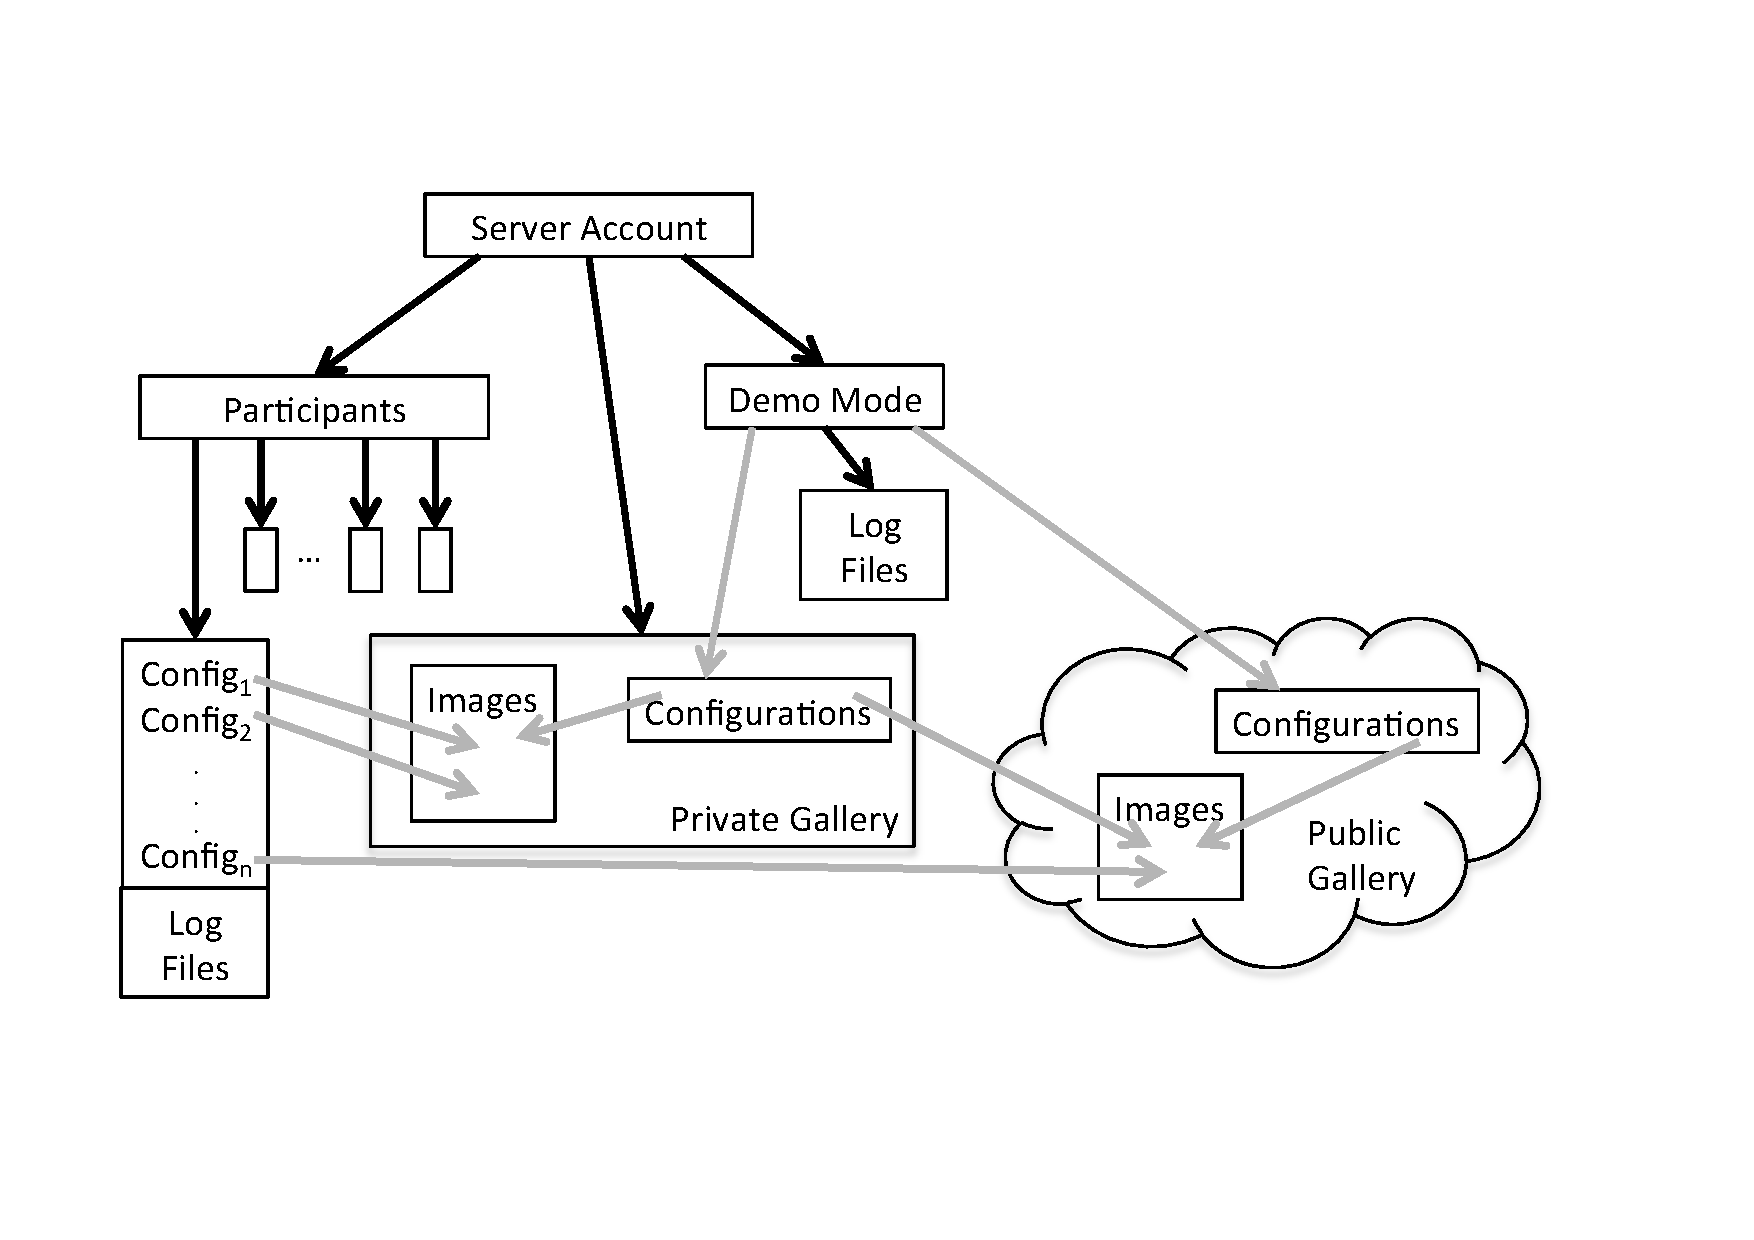
\includegraphics[scale=0.6]{Overview3_cropped.pdf}

\caption{\label{fig-overview}Overall structure of data in PsyPad.
Having a server account allows access to all of your own 
participants, configurations and images, in addition to Demo Mode
and the Public Gallery of images and configurations.
Each entry in the image library is a zip file of images as per
Section~\ref{sec-images}. Each participant has their own local copy
of configurations named ``Config$_x$'' in this figure (see Section~\ref{sec-tests}), 
which may or may not be replicated in the either of the galleries.
Log files (Section~\ref{sec-logs})
are attached to participants, or the Demo Mode, and never feature 
in the galleries.
Each test configuration uses one of the image sets in
the from either gallery. 
}

\end{center}
\end{figure}

\section{Gallery}

Figure~\ref{fig-overview} shows the overall structure of the PsyPad server.
The collection of tests and
stimuli are split into public and private galleries.


\subsection{Public gallery}
\label{sec-publicGallery}


We provide a collection of test configurations and image sets in the public gallery that you can download and run in
Demo mode (see Section~\ref{sec-demoMode}), or add to your own 
participants (see Section~\ref{sec-importingFromGallery}). You can submit any configurations you create (see Section~\ref{sec-creatingConfigurations}) for consideration to be added to the public gallery (see Section~\ref{sec-submittingConfigurations}).

The public gallery can be accessed on the server by going to the [Configuration Gallery] (for public configurations) or [Image Sets] (for public image sets) tab and selecting the [Public Configurations] or [Public Image Sets] option.

\subsection{Private gallery}
\label{sec-privateGallery}

Your private gallery can be accessed on the server by going to the [Configuration Gallery] (for configurations) or [Image Sets] (for image sets) tab and selecting the [Private Configurations] or [Private Image Sets] option.

Configurations and image sets you upload to your private gallery can not be seen by other PsyPad users (see Section~\ref{sec-server} for security disclaimers).


\section{Participant mode}
\label{sec-participantMode}

As opposed to Demo mode, Participant mode allows you to configure experiments for participants
where multiple experiments can be presented sequentially with the
results uploaded to the server on completion.

You can switch to Participant mode from Demo mode by pressing
[Configure PsyPad] and pressing the green toggle next to ``Demo Mode".
When doing this, \textcolor{red}{ensure you know the admin password (if it is set)} so you can return to
the admin panel later.

To return to the admin panel from Participant mode,
enter 'admin' as the participant name followed by the password (of it has been 
set in the admin panel).
If you forget this password you will need to uninstall and reinstall
the iPad app.

Participants need to be configured on the server (see Section~\ref{sec-configuringParticipants}).

To run a test in Participant mode, close the admin panel if it is open,
enter the participant username then press [Login].
From there you will be able to press [Begin Test] or [Begin Practice
Test] (visible if any practice tests are configured).
Once the test is completed, the logs will be automatically uploaded to
the server if there is an internet connection available.

When you press the [Login] button the latest version of the participant configuration will be downloaded if there is an internet connection available.

\subsection{Pre-downloading participant configurations}

It is recommended to download participant configurations before beginning tests,
especially if the configuration uses large image sets.
It is also necessary if there will be no internet connection available
where the test is run.

To pre-download a participant's configurations, open the admin panel, press 
[Load server participant list] then press the [Download] button next to a participant.

You can also simply log in as a participant to ensure their configuration is downloaded.

\section{Internet connection}

All tests undertaken are logged in both Demo and Participant mode.
If there is an internet connection present at the end of a session, the
the log file for that session, and any previous sessions that have not
been uploaded, will be uploaded to the server.

If an internet connection was not present at the end of a session, you
can upload the logs at a later date by pressing [Upload logs to server]
in the admin panel, or wait until the end of another session performed
by that participant when an internet connection is present.

See Section~\ref{sec-logs} for more information on logs.

If an internet connection is present when a participant logs in to
PsyPad, their configurations are downloaded from the server.
If there are new configurations that use images sets that are not
already on the iPad, these are also downloaded.

This allows remote altering of participants' testing parameters when an iPad is `in the field'. You may want to consider using an iPad with a SIM card on an active data plan if you need to ensure internet connectivity.

\section{Adding and configuring participants}
\label{sec-configuringParticipants}

When the iPad app is in Participant mode, participants will need to enter in their username before each session. You might want to choose usernames that are easy to type on the iPad. Participants have both configurations and logs associated with them.

\subsection{Participant list}

You can view a list of participants on the server by selecting the [Participant] tab.

From there you can create a new participant by clicking [New
Participant].
Choose a username and click [Create Participant].

From the participant list you can click on the link in the Configurations column 
to access
a participant's configurations and the link in the Logs column to access their test logs
(Section~\ref{sec-logList}).
You can click on [Edit] to change their username, 
and [Delete] to delete them.

\subsection{Participant log list}
\label{sec-logList}

Clicking on a link in the Logs column in the participant list will take
you to a list of the participant's logs.
From there you can [View] and [Delete] logs.
You can filter the log list using the filter options on the right and
you can download the logs in various formats using the download links
at the bottom left of the log list.

\subsection{Participant configuration list}
\label{sec-configList}

Clicking on a link in the Configurations column in the participant list
will take you to a participant's configuration list.
From there you can [Edit], [Delete], [Save to Gallery] and
[Duplicate] configurations.

You can also create a [New Participant Configuration]
(Section~\ref{sec-creatingConfigurations}) or [Import from Gallery]
(Section~\ref{sec-importingFromGallery}).

\subsection{Importing configurations from the gallery}
\label{sec-importingFromGallery}

Clicking [Import from Gallery] in a participant's configuration list will take you to the import screen. From here, select the configurations you would like to import from the gallery. Select whether or not you want to overwrite existing configurations then click [Import From Gallery].

Selecting ``Yes" for ``Overwrite existing configurations" will mean that any configurations that the participant already has with the same name as a configuration you are importing will be overwritten. This allows you to update a configuration in your gallery (see Section~\ref{sec-privateGallery}) and import the changes you make to multiple participants.

\subsection{Exporting configurations to the gallery}

Clicking [Save to Gallery] in a participant's configuration list will
take you to the export screen.
You may be presented with the option to overwrite existing
configurations if there are any configurations in your private gallery
with the same name.
To perform the export, simply click the [Save to Gallery] button.

To copy configurations from one participant to another, you should use the gallery as a ``clipboard''. Copying to the
gallery also allows the configuration to be used in Demo mode.


\section{Creating your own test configurations}
\label{sec-creatingConfigurations}

Configurations can either be created in your private configuration gallery (see Section~\ref{sec-privateGallery}) or created for an individual participant. Note that you can save participant configurations to your gallery, and you can import configurations to a participant from the gallery. This mechanism allows you to create a configuration in your gallery that can be imported and used by multiple participants.

Only configurations in the gallery will be accessible from Demo mode (see Section~\ref{sec-demoMode}).

To create a configuration in your gallery, click on the [Configuration Gallery] tab then click [New Gallery Configuration]. To create a configuration for an individual participant, click on [New Participant Configuration] in a participant's configuration list (Section~\ref{sec-configList}).

There are two parts to creating your own test configurations. Firstly, you need to create or select an image set to use. Secondly, you need to specify the test parameters.

There are pre-made image sets available in the public gallery (Section~\ref{sec-publicGallery}) that you can use, though you will first need to understand the image set folder structure. For an explanation of the folder structure and instructions on how to create your own image sets, see Section~\ref{sec-images}.

For a breakdown of the test configuration options, see Section~\ref{sec-configs}.

Once you have selected the image set and set the configuration options, click [Create configuration] at the bottom of the page to create the configuration.

\subsection{Things to consider for your test configurations}

\begin{enumerate}

\item {\bf Stimuli.} All stimuli in PsyPad are precomputed 
24- or 32-bit PNG
images that are presented centred on the screen, and written over a background image that is also a PNG.
Dynamic stimuli are a sequence of frames that are also
PNG images.  The filenames of the images must be in
a specific format: see Section~\ref{sec-images}.
If you cannot precompute all the stimuli you might need in a test, then
PsyPad will not work for you.

\item {\bf Buttons.} What response buttons do you need for your test?  
Up to four
rectangular buttons are allowed. Where
should they be placed on the screen? 
What color, width and height
should they be?

\item {\bf Thresholding strategy: MOCS or staircase?}
If you choose a MOCS, you must decide on the stimuli levels you want to
test, and how many trials per level: see Section~\ref{sec-mocs}.
For staircases, you must decide how many to interleave; and for each the starting
values, the number of reversals, and the step sizes between each reversal.
See Section~\ref{sec-staircase} for more information.

\item {\bf How many tests in a session?}
Does a session (from participant login on the iPad
to completion of all tests) consist of just one
test (a thresholding run for one stimuli type), or do you want more than one test
in a session?  What order do you
want the tests? Do you want different tests on different days of the week?
Do you want a different random seed for each test?
See Section~\ref{sec-configs} for information on how to set up tests.

\item {\bf Do you want a practice session?}
If you mark some test configurations as ``Practice configurations'', then 
once a participant logs in to PsyPad, there are options 
to [Begin Test] and [Begin Practice Test].
The practice test session can be configured separately 
from the main test session, but otherwise shares all features with 
main test sessions. Practice sessions are identifiable as such in log
files.

\end{enumerate}

\subsection{Submitting to the public gallery}
\label{sec-submittingConfigurations}

We would love to let you share configurations/image sets that you think would be helpful for other people to use.

If you would like to submit a configuration (and its image set) for
consideration to be added to the public gallery, simply click on [Share
to Public Gallery] on a configuration list.
We will review any submitted configurations and let you know via email
if we add them to the public gallery.


\section{Image Stimuli}
\label{sec-images}

\begin{figure}
\begin{center}
\subfigure[]{\qquad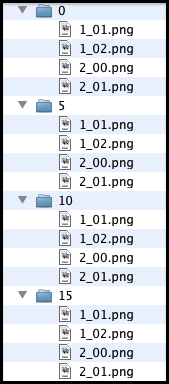
\includegraphics[scale=0.5]{SimpleImageHeirachy}\qquad}
\subfigure[]{\qquad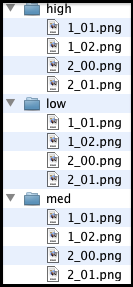
\includegraphics[scale=0.5]{SimpleImageHeirachy_MOCS}\qquad}
\subfigure[]{\qquad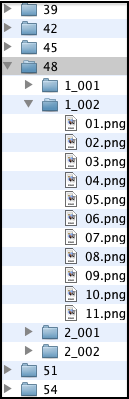
\includegraphics[scale=0.5]{SimpleImageHeirachy_Movie}\qquad}
\caption{\label{fig-egImages}Folder and image filenames for (a) a staircase or MOCS 
procedure that has stimuli levels 
$\{0,5,10,15\}$; (b) a MOCS with three levels {\tt low}, {\tt med}, and {\tt high}; and 
(c) a movie stimulus with levels $\{39,42,\ldots,54\}$.
In (a) and (b) the prefix of the filenames give the button number for a correct response (1 or 2), and
(c) the same is given by the prefix of the subfolder name.
In (c), files are movie frames that are presented in lexicographic sequence.
}
\end{center}
\end{figure}

%\caption{\label{fig-egImages}Image filenames for a MOCS procedure with
%three stimuli levels ({\tt low}, {\tt med}, and {\tt high}, and four
%(presumably different) images at each level. For each presentation of
%one of the levels, a random image from the four possible is chosen.


All stimuli in PsyPad are 24-bit RGB PNG images 
(\url{www.libpng.org/pub/png/}) which
are presented without alteration in the centre of the screen.
You can generate these any way you
like (ImageMagick, Photoshop, Matlab, R, custom C code, etc), but 
their folder/directory location and filenames are
important.
PsyPad will also faithfully display 32-bit RGBA PNG images if
you want to make use of the Alpha channel for transparency.

The thresholding algorithms in PsyPad identify stimuli using folder
names (not image filenames).  This allows for different random
images of the same stimulus level to be used by PsyPad.
For example, when PsyPad is asked to present a stimulus
of level 33, it randomly selects an image from the folder named 33.

Each stimuli folder must be named in
the correct format for the thresholding algorithm that you chose:
\begin{itemize}
    \item any alphanumeric text, if a MOCS is to be used; or
    \item an integer corresponding to stimulus level, if a staircase thresholding algorithm is to be used.
\end{itemize}

Note that because PsyPad's staircases work on integer stimuli levels, you may have to
be a little creative in mapping your thresholding domain onto an integer
domain. For example, if you are thresholding in log units with a
step size of 0.2 log units, you might convert a stimulus level $\ell$ to
the integer $\lfloor 1000\times 10^{-\ell} \rfloor$, giving stimuli levels
of 
$\{6,10,15,25,39,63,100,158,251,398,630,1000\}$.

Inside each folder, the images themselves must be named in a 
specific format, as described in Sections~\ref{sec-single-frame} and~\ref{sec-multi-frame}.

\subsection{Single frame images}
\label{sec-single-frame}

Within the folder, individual images must be named as 
\begin{center}
  $b$\_$n$.png
\end{center}
where $b$ is the button number that would correspond to a ``correct''
response for this stimuli, and $n$ is an integer.
See Figure~\ref{fig-egImages}(a) for an example.
The button numbers are used to generate a test summary on the iPad for 
the ``admin'' user
(see Section~\ref{sec-onIpadAnalysis}), 
and to determine correctness for each step in staircase procedures. 
If you do not follow this naming convention, staircases will not work, and 
on-iPad analysis will not work.

While folder names in the format for a staircase also match the 
requirements for 
a MOCS, the folder names for a MOCS can be more general; for example
as in Figure~\ref{fig-egImages}(b).



\subsection{Multiframe images (movies)}
\label{sec-multi-frame}

Dynamic stimuli are achieved using a sequence of frames that are also
24-bit RGB PNG images (or 32-bit RGBA) but in a subfolder named as for the single 
images without the {\tt .png} suffix, with the individual frames 
named in lexicographic order (for example, 11 comes before 2.) If you want
numeric order, make sure you pad with leading zeroes as in Figure~\ref{fig-egImages}(c),
which shows 
stimulus level 48 consisting of 11 frames where a button
press of 1 would be ``correct''.

The time that each frame of the movie is displayed before the next frame is
presented and the looping behaviour is set as part of the test configuration;
see Section~\ref{sec-tests}.

\subsection{Background Image}
\label{sect-bi}

As of Version 1.1 of the PsyPad app, you can also include a background
image that is displayed centred on the screen throughout the entire
test, with stimuli and buttons written over the top of that image.
This is useful for fixation targets, in particular, but could also
be used in many creative ways.  The background image must be a PNG,
and must be named {\tt background.png} in the top directory/folder
of images.  The screen is always set to the background color and
overlaid with the centered background image, so if no {\tt
background.png} is present the screen appears as the background
color.

To avoid apparent flickering of buttons, the background image should
either contain the buttons in the actual image, or be small enough
to not overwrite the buttons when the display is refreshed.

\subsection{Gamma correction and Auto-brightness}

There is no Gamma correction or look up table (LUT) capabilities in PsyPad.
You need to do your own gamma correction and luminance determination offline, and then
choose the pixel values in your images accordingly.
For example, there is no guarantee that RGB$=(127,127,127)$ 
is mean luminance on every device. If
exact luminance is important to you, you should use a photometer and measure different
pixel levels, and make your images accordingly.

PsyPad sets the iPad to maximum brightness at the beginning of a
test session, but cannot control the ``Auto-Brightness'' setting.
You should make sure this is off, and instruct participants never
to turn it on, if luminance levels are important to your test.

For calibration, you can create an image set that contains 
a set of ``blanks'' which contains full size images 
all of one pixel level. It might be easiest to annotate each corner of the
image with the pixel value, too.
You can then set up a MOCS or staircase using this image set 
to aid in calibration.

\subsection{Ramping} 

Images are not ramped, and are presented
immediately after the inter-stimulus interval expires.  
If you want to ramp your stimuli on and/or off, make a movie style
image that contains the ramp you require.

\subsection{Timing} 

We do not have program access to the ``graphics clock'' on the iPad,
and so very precise frame presentation times are not supported.  If
you require very fine timing control of stimuli presentations, then
PsyPad is probably not for you.  We have endeavoured to be as
accurate as possible with presentation and inter-stimulus interval
timing, and it should be sufficiently accurate for most tests.

\subsection{Uploading the images}

Image sets must be uploaded separately before you can associate them with a test configuration.

Once you have all the images you need for a single test, named correctly,
you should zip them all into a single zipfile without an enclosing folder (using {\tt zip} on MacOS or Linux, or {\tt winzip} on Windows) and upload them to the server by selecting the [Image Sets] tab and clicking [Import Image Set].

They will then be automatically processed on the server and put in a suitable format (a single big file with an index) for transfer to the PsyPad iPad app. When PsyPad is next started with an internet connection to the server, and a participant using the image set logs in, the images will be transferred and stored on the iPad. This might take a while, so it is recommended that you log in as at least one participant using the 
image set so that this download is already done before the actual participants
use the app.

\section{Test configuration options}
\label{sec-tests}

In order to define a test you need to choose an image set already
uploaded to the server (see Section~\ref{sec-images}) and then choose
several options as described in this table. This table lists the
options in the order they appear on the server interface.

To preview the background colour, exit button and response buttons as they will appear on the iPad (not 100\% accurate), click [Show Preview] at the bottom right of the browser window.

\begin{longtable}{|p{5cm}|p{10cm}|}
\hline
{\bf General Settings}  & \\\nopagebreak
\hline
Name & Simply identifies the test configuration, for your organisational use only. Does not have to be unique, but might be easier for you if it is. When importing configurations from the gallery or exporting to the gallery, this name affects the optional overwriting behaviour (see Section~\ref{sec-importingFromGallery}). \\
\hline
Title & This text appears on the iPad along with a {\tt Begin} button
before the test.
You might like to put something here that reminds the participant of
the task.
\\
\hline
Description & For your organisational use. Be descriptive here if you are considering submitting this to the public gallery.\\
\hline
Enabled & If true, then this test is part of a participant's session\\
\hline
Is Practice Configuration & If true, then this test is part of a participant's practice session (if also ``Enabled''). Practice configurations are started by pressing [Begin Practice Tests] instead of [Begin Tests] on the iPad.\\
\hline
Order & This specifies the order in which this test will appear in 
the session (if enabled). Any integer is fine: the tests are sorted by this number to get their order for a session.\\
\hline
Days of the week & The test configuration will only be enabled 
on the selected days of the week.\\
\hline
\hline
{\bf Image Sets}  & \\\nopagebreak
Image Set & Choose from the image sets in the public and private image set gallery.\\
\hline
Loop animations & Only relevant for images that are a sequence of frames (movie). If true then the frames loop until a button is pressed.\\
\hline
Animation frame rate & This is the number of frame refreshes on the iPad
for which each image in the movie sequence should be displayed.
Currently iPads have a frame rate of 60Hz.
For example, if you want a movie of 8 images to display for 400 ms, you
would enter 3 here. ($3/60\times 8 = 0.4$.)
\\
\hline
\hline
{\bf Staircase Method Parameters}  & \\\nopagebreak
Use staircase method & If Yes, then staircase is used, otherwise MOCS. \\
\hline
Number of staircases & The number of
staircases you wish to interleave (should be at least one) \\
\hline
Start level & A list of start levels separated by a ``/'' character; one for each staircase
            (each must match a filename of an image as per Section~\ref{sec-images}) \\
\hline
Number of reversals & A list of the number of reversals before terminating the staircase 
            separated by a ``/'' character; one for each staircase. \\
\hline
Floor/ceiling hits to finish & A list of the number of times the minimum/maximum stimuli are shown
            before terminating the staircase 
            separated by a ``/'' character; one for each staircase. \\
\hline
Minimum level & The minimum stimulus level 
            separated by a ``/'' character; one for each staircase
            (each must match a filename of an image as per Section~\ref{sec-images}) \\
\hline
Maximum level & The maximum stimulus level 
            separated by a ``/'' character; one for each staircase
            (each must match a filename of an image as per Section~\ref{sec-images}) \\
\hline
$\Delta$ values & The step sizes before each reversal as a comma separated list
            separated by a ``/'' character; one for each staircase
            (must be the same number as in ``Number of reversals'' for each staircase)\\
\hline
\# wrong to get easier & The number of ``incorrect'' responses before 
            the stimulus level is increased
            separated by a ``/'' character; one for each staircase. 
            Note
            that an incorrect response adds the current step size to the 
            current stimuli level.\\
\hline
\# correct to get harder & The number of ``correct'' responses before 
            the stimulus level is reduced
            separated by a ``/'' character; one for each staircase.
            Note
            that a correct response subtracts the current step size from the 
            current stimuli level.\\
\hline
\hline
{\bf MOCS Parameters} & \\\nopagebreak
\# questions per folder & A comma separated list of pairs of the form $s:n$, where $s$ is the stimulus
level (matching the filename of an image in the chosen image set) and $n$ is the number of trials. For
example, $16:40,18:40,20:40$ is a MOCS over three stimuli levels 16, 18, and 20 using 40 trials for
each level.\\
\hline
\hline
{\bf Display Configuration} & \\\nopagebreak
Background color & An RGB-hex string beginning with a \#. For example, \#FF0000 is red. This is the
color of the screen when the {\tt Begin} button is displayed, between stimuli, 
    if the {\tt Next} button is used, 
and also as the background for your images if they do
not fill the entire screen or contain transparent pixels.\\ 
\hline
Show exit button & If ``Yes'' then a small cross is displayed as per the exit position given below.\\
\hline
Exit button position & $(x,y)$ width and height
of the exit button. All measurements are in pixels, the top left of the screen is $(0,0)$, and the bottom right is $(1024,768)$.\\
\hline
Exit button color & Background and foreground colors as RGB-hex strings. For example, \#00FF00 is
green. Ignored if ``Show exit button'' is ``No''. You can preview the position and colour of the exit button by clicking [Show Preview] at the bottom right of the browser window (not 100\% accurate).\\
\hline
\hline
{\bf Button Configuration} & \\\nopagebreak
Number of buttons & The number of response buttons (maximum 4). From Version 1.1 onwards, 
if only one button is chosen, if it is pressed within the response window this counts as a ``correct'' response,
otherwise it counts as an ``incorrect'' response.\\
\hline
Button text & The text to appear on each button\\
\hline
Button presentation delay & The amount of time (in seconds) before the buttons appear after the stimuli has been presented (does not have to be an integer)\\
\hline
Button backgrounds & RGB-hex string specifying the background color of each button. For example,
\#0000FF is blue.\\
\hline
Button text colours & RGB-hex string specifying the text color of each button. For example,
\#888888 is grey.\\
\hline
Button positions & For each button, $(x,y)$ width and height.
All measurements are in pixels, and the top left of the screen is $(0,0)$,
and the bottom-right is $(1024,768)$ (even on iPad III). You can preview the position, colour and text of the buttons by clicking [Show Preview] at the bottom right of the browser window (not 100\% accurate).\\
\hline
\hline
{\bf General Test Parameters} & \\\nopagebreak
{\tt Next} button after each response & If ``Yes'' then a {\tt Next} 
            button appears after each response
            and must be pressed before the next trial begins.\\
\hline
Time between each question & Specify the mean time between response button press and the variation.
The next stimuli is presented after $\mbox{mean}\pm\delta$ where $\delta$ is sampled uniformly at
random from $[-\mbox{variation},\mbox{variation}]$. \\
\hline
Infinite presentation time & If ``Yes'', stimuli are presented until a button is pressed; 
otherwise if ``No'' you must specify the presentation 
time in seconds. In the ``No'' case, the image is replaced with the background color
and background image (if present, Version 1.1 onwards) and the buttons remain. 
This option can interact strangely with movie stimuli. 
If you have chosen Yes, and have a movie stimuli that is not looping, you will get the background
color (and background image if specified) 
once the movie runs out of frames. If you have chosen ``No'' and a value that is shorter than 
the movie (number of frames $\times$ frame rate/60) then the movie will be truncated.\\
\hline
Infinite response window

\vspace{2ex}
(This option is not used in PsyPad App Version 1.0.) 
&
If ``Yes'' then PsyPad will wait until a button is pressed before proceeding to the next
stimuli.
If ``No'' you must specify a time in seconds. If a button is pressed 
within this time (started from stimulus onset),
then PsyPad will proceed to the next stimuli, checking the button number against the image file name for
``correct'' or ``incorrect''. If there is only one button, and it is pressed within the window, a ``correct'' response
is recorded.
If ``No'' and a button is not pressed pressed within the time limit (from stimulus onset), then 
an ``incorrect'' response will be recorded.\\
\hline
Use specified seed & If ``Yes'' the provided number is used to seed the random number generator (handy
for testing so that you get the same image sequences); otherwise if ``No'' a random seed from
{\tt /dev/urandom} is used.\\
\hline
Attempt facial recognition & If ``Yes'' then a picture is taken with the on-board camera at the
beginning of every stimulus presentation (beware of the camera ``noise'' that can be turned off on the
iPad Settings). The image is processed to locate two eyes and a mouth. The three coordinates are saved
into the log file. If ``No'', no picture is taken, and nothing is logged.\\
\hline
\end{longtable}

After choosing all of your settings, don't forget to save the configuration using the appropriate button at the bottom of the screen.

\subsection{MOCS}
\label{sec-mocs}

To set up a MOCS procedure you need the stimuli levels to test, and the
number of trials per level.
Once you have chosen your image set to use as the basis for your test,
the levels are defined by the folder names in your image set.
For example, if you used the image set from Figure~\ref{fig-egImages}(b),
the test levels are {\tt low}, {\tt med} and {\tt high}.

On the server, the number of trials per level to use is specified in 
a comma separated list as
$$
{\ell_1}{:}{n_1}{,}{\ell_2}{:}{n_2}{,}\ldots
$$
where $\ell_i$ is the stimulus level matching the folder names, $n_i$ is the number of trials at that
level.
On the iPad, the interface for specifying these is a bit nicer as it lists all available levels, and
you enter the number of trials next to each level (leave blank for no trials.)
Remember if you alter tests on the iPad to upload them to the server before a participant logs in,
otherwise the server version will overwrite your changes (if an internet connection is present.)

For the example in Figure~\ref{fig-egImages}(c), if you want 10 trials per level you would use the
following string.
$$
\mbox{\tt low}{:}10{,}\mbox{\tt med}{:}10{,}\mbox{\tt high}{:}10
$$

The order of levels is chosen at random, and images within each level are chosen at random without
replacement (unless the number of trials exceeds the number of images, in which case some images will
be repeated $\lceil\mbox{images}/\mbox{trials}\rceil$ times.)

\subsection{Staircase}
\label{sec-staircase}

A correct response (as determined by matching the first character of the 
filename of the stimulus with the button number pressed) will cause the
current step size to be subtracted from the current stimulus level to
determine the next stimulus level to display.
An incorrect response 
will cause the
current step size to be added to the current stimulus level.

Thus, PsyPad assumes ``hard to see'' stimuli have higher folder numbers than ``easy to see'' 
stimuli.
If you prefer working in a reverse scale (eg dB where a low number is ``easy'' and a high number ``hard'')
you can always reverse the button labels on your images, so that
when the participant press the correct button, you treat it as incorrect for the purposes of the 
staircase.

A reversal is registered whenever the number of wrong/correct in
a row is recorded followed by the number of correct/wrong in a row.
For example, in a 1-up, 1-down staircase 
({\tt \#wrong}=1, {\tt \#correct}=1),
a correct followed by an incorrect or vice versa is a reversal.
In a 1-up, 2-down staircase
({\tt \#wrong}=1, {\tt \#correct}=2), then reversals would be triggered by
responses incorrect-correct-correct and correct-correct-incorrect.

Each staircase terminates when its number of reversals is achieved, or 
if the count of minimum/maximum stimulus value correct/incorrect reaches 
the specified number.

\section{Session Configurations}
\label{sec-configs}

A session is simply a list of enabled tests, which are executed in
order. If you want different tests on different days of the week,
you should make sure that all the tests for all days are enabled,
and then each test is configured for the appropriate day.

Note that the practice session is separate from the test session,
and so if you want the same test to appear in both, you need to
duplicate the test and set the {\tt Is practice configuration} option in the duplicate.

\section{Server Setup}
\label{sec-server}

\subsection{The PsyPad.net.au Server}

Note that while \defaultServer is password protected, and under 
normal circumstances
your log files are not available to any other users, we are not providing
a state-of-the-art secure environment. Any determined hacker will be able to 
get access to your logs in much the same way as they 
can access your personal computer,
iPad, etc, despite our best efforts.
We also have administrator access to your logfiles. 
While we have procedures in place to
limit the use of this access, we may inadvertently view 
your logs while maintaining or
updating the system. 
As such, {\bf do not include any private or unethical data in
your participant identifiers or image file names 
that will appear in the log files.}

Note that this standard level of security does not compromise your
research as log files only contain sequences of image names and
button responses. There is no easy way for an outside observer 
to tell what the stimuli are, or
to which images filenames correspond.

While the server is currently backed up weekly, do not rely on this for your
data persistence.
Make your own backups of log files using the {\tt Export all logs} 
regularly. 

\subsection{Your Own Server}
\label{sec-ownserver}

The source code for the server (implemented with Ruby on Rails) is available at \url{https://www.github.com/davidlawson/PsyPad-Server}, but it requires some technical expertise to deploy. We do not plan to support you in running your own server.

\subsection{Communication with iPad}

\subsubsection{Automatic session transfer from Server to iPad}

When a participant logs on, and an internet connection is available to PsyPad, 
their session information is checked against the server, and if updated the
new version is downloaded. This allows remote altering of session configurations. 

\subsubsection{Log file transfer from iPad to Server}

This happens automatically at the end of a session if there is an internet
connection, and is never repeated (if successful).
The ``admin'' user on the iPad can force the sending of all 
log files by pressing [Upload logs to server] on the Admin Panel.

\section{Handling Logfiles}
\label{sec-logs}

Logfiles contain lines of text with three columns delimited by a vertical bar (pipe) symbol. The fields are
\begin{enumerate}
    \item time stamp (in number of seconds since 1/1/1970); 
    \item identifier that describes the line; and
    \item the data related to the identifier.
\end{enumerate}
Figure~\ref{fig-exampleLog} shows an example log file for a staircase procedure, and Table~\ref{tab-logs} describes each
identifier.
The log file format has been designed for processing with script languages such as awk, Perl, Python, and so on. The
\defaultServer server offers the summary text. 
Example Python scripts for processing logfiles can be found in the Gallery at \defaultServer.

\begin{figure}
\begin{center}
\begin{verbatim}
 Summary                            1378869851|test_begin|...
 Test date: 11/9/2013 13:24:11      1378869851|next_question|1
 Glass staircase                    1378869851|currentStaircase|0
 Practice: no                       1378869851|currentReversal|0
 Staircase: 0                       1378869851|presented_image|50/2_005.png
     Not seen max: 0                1378869851|presented_buttons|Concentric Radial 
     Seen min: 0                    1378869852|image_hidden|(null)
     Reversal 1: 58                 1378869859|reaction_time|7711.23ms
     Reversal 2: 54                 1378869859|button_press|1 (Concentric)
     Reversal 3: 58                 1378869860|next_question|2
     Reversal 4: 52                 1378869860|currentStaircase|0
     Reversal 5: 54                 1378869860|currentReversal|0
     Reversal 6: 52                 1378869860|presented_image|58/2_003.png
 Start time: 11/9/2013 13:24:11     1378869860|presented_buttons|Concentric Radial 
 End time  : 11/9/2013 13:24:55     1378869860|image_hidden|(null)
 Duration  : 0 minutes 44 seconds   1378869861|reaction_time|1820.66ms
                                    1378869861|button_press|2 (Radial)
                                    ...
                                    1378869890|reversal|(null)
                                    1378869891|next_question|16
                                    1378869891|currentStaircase|0
                                    1378869891|currentReversal|5
                                    1378869891|presented_image|52/1_002.png
                                    1378869891|presented_buttons|Concentric Radial 
                                    1378869891|image_hidden|(null)
                                    1378869892|reaction_time|1424.79ms
                                    1378869892|button_press|1 (Concentric)
                                    1378869893|next_question|17
                                    1378869893|currentStaircase|0
                                    1378869893|currentReversal|5
                                    1378869893|presented_image|52/1_001.png
                                    1378869893|presented_buttons|Concentric Radial 
                                    1378869893|image_hidden|(null)
                                    1378869895|reaction_time|1773.27ms
                                    1378869895|button_press|2 (Radial)
                                    1378869895|reversal|(null)
                                    1378869895|test_finished|(null)
                                    1378869895|exit_test|(null)
\end{verbatim}
\caption{\label{fig-exampleLog}An example logfile for a staircase procedure (right), and a summary of that logfile (left).
}
\end{center}
\end{figure}


\begin{table}
\begin{center}
\begin{tabular}{llp{10cm}}
\hline
Identifier & Data type & Meaning \\
\hline
button\_press       & $d$ (String) &  The number and text on the response button that was pushed. \\
currentReversal     & $d$ & The number of reversals seen so far. (Staircase only)\\
currentStaircase    & $d$ & The current staircase being presented. (Staircase only)\\
exit\_test          &  --  & Last line in a single test log. \\
image\_hidden       &  --  & Time image was replaced with background. \\
next\_question      & $d$ & The question number in the current test. (Staircase only)\\
next\_question      & $d$/$d$ & The question number in the current test (numerator) 
                                and the total number of questions (denominator). (MOCS only)\\
presented\_buttons  & String & Labels of each button presented for this question. \\
presented\_image    & String & Filename of image that was presented at this time. \\
reaction\_time      & $d.dd$ms & Time between image presentation and button push. \\
reversal            & -- & This response caused a reversal. (Staircase only) \\
test\_begin         & String & Description of all test parameters in JSON format. \\
test\_finished      &  -- & Time the test finished.\\
distance\_detection & String & Result of face detection (if turned on). 
                    An example string is {\tt Question 5: Detected facial 
                    features: left eye 733.75/443.75, right eye: 932.50/482.50,
                    mouth: 876.25/236.25}, where each number pair is the x/y 
                    coordinate of the preceding feature.\\
\hline
\end{tabular}
\caption{\label{tab-logs}An example logfile for a staircase procedure (right), and a summary of that logfile (left).
$d$ indicates an integer and $d.dd$ indicates a decimal number.
}
\end{center}
\end{table}



\section{Checking test results on the iPad}
\label{sec-onIpadAnalysis}

\begin{figure}
\begin{center}
\subfigure[]{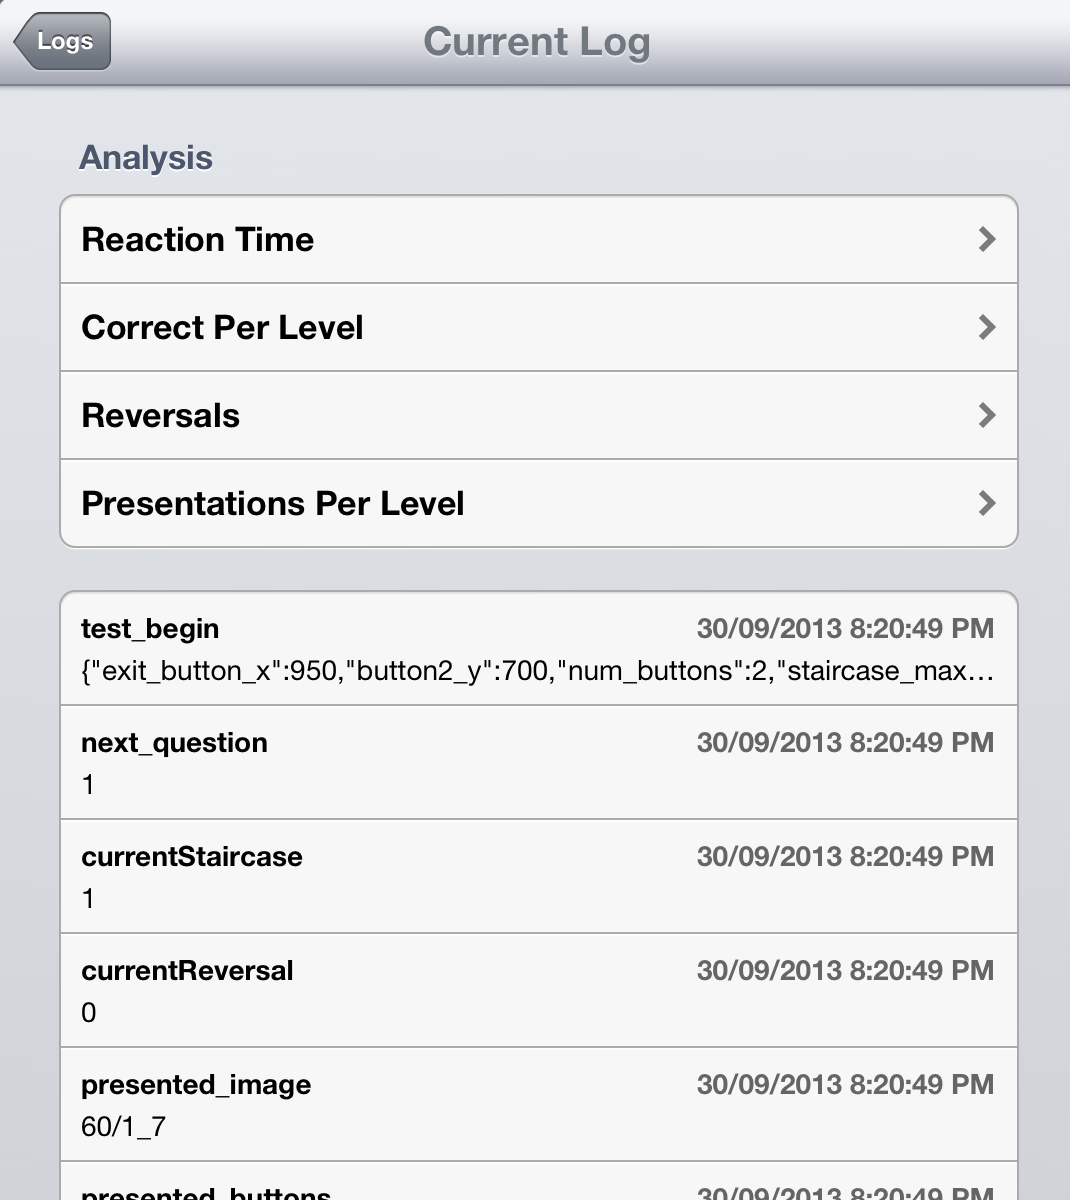
\includegraphics[scale=0.15]{screenshots/viewlogCrop}}
\subfigure[]{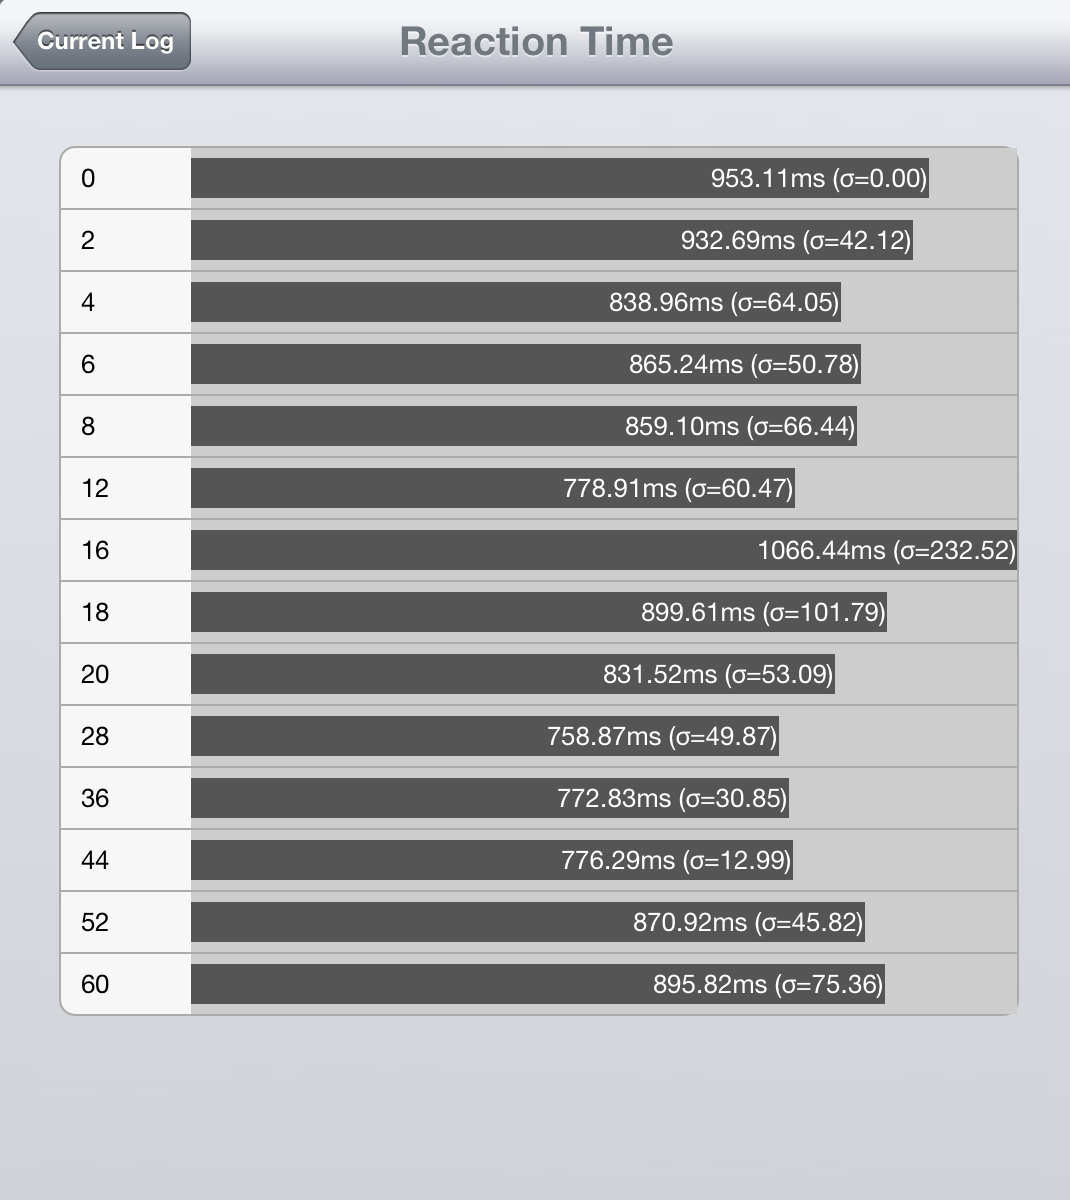
\includegraphics[scale=0.15]{screenshots/reactionTimeCrop}}
\subfigure[]{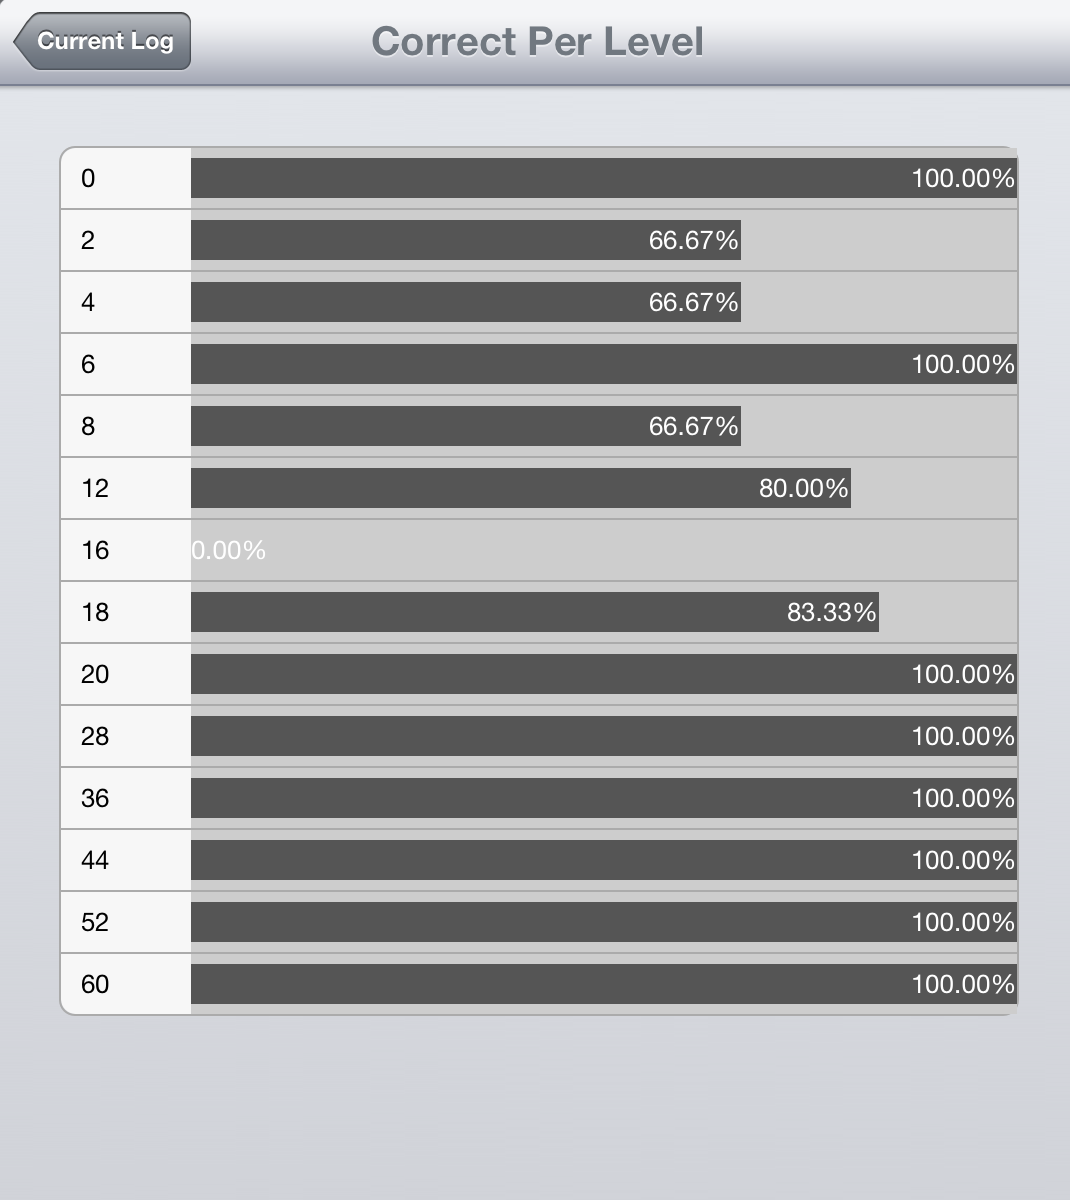
\includegraphics[scale=0.15]{screenshots/correctPerLevelCrop}}
\subfigure[]{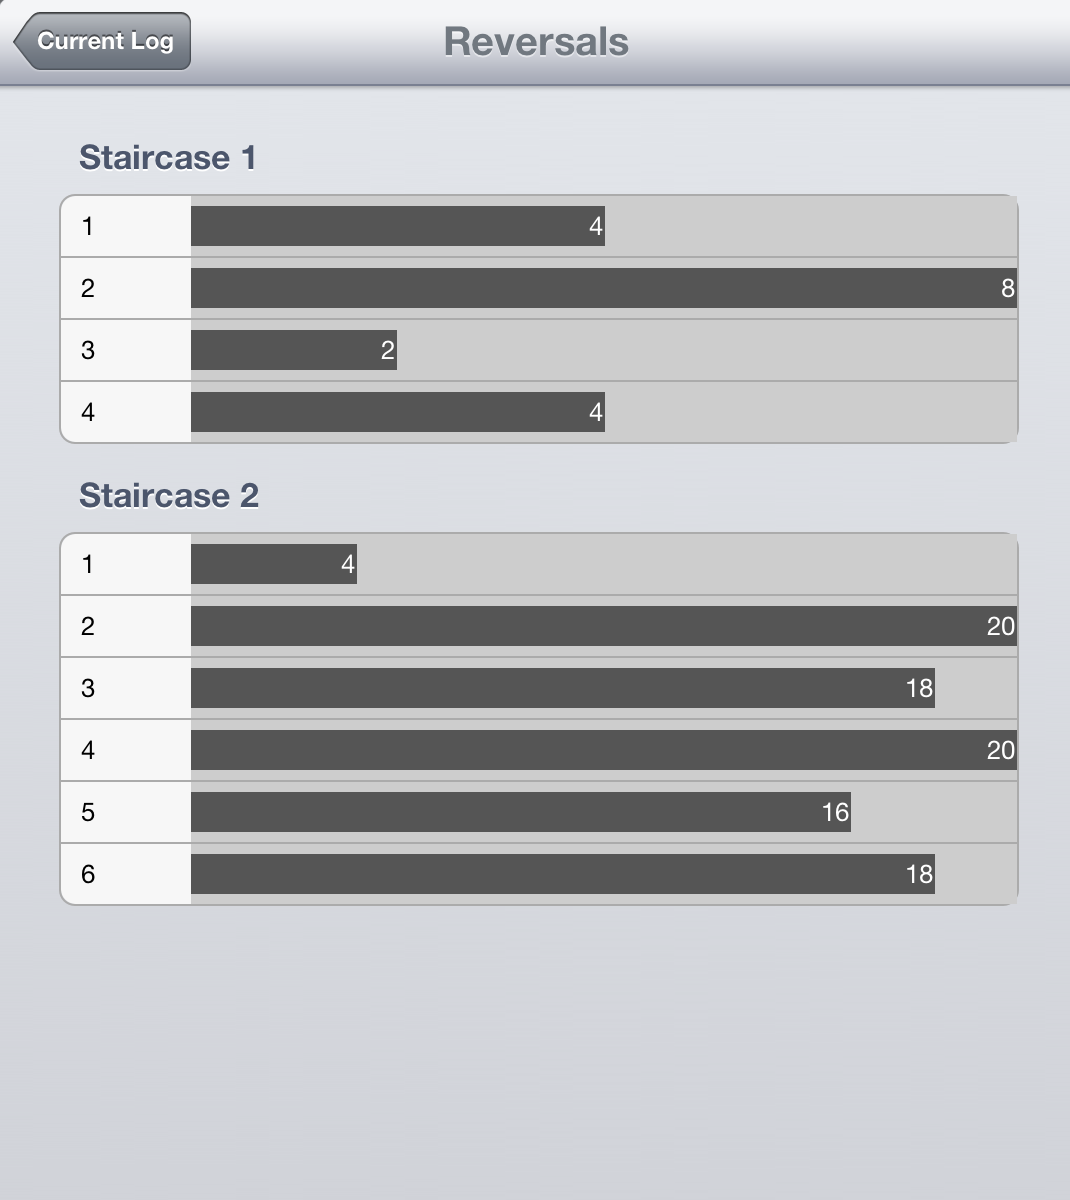
\includegraphics[scale=0.15]{screenshots/reversalsCrop}}

\caption{\label{fig-anal}Overall structure of data in PsyPad.
An administrator owns an image library and a list participants.
Each entry in the image library is a zip file of images as per
Section~\ref{sec-images}. Each participant has a list of test
configurations named ``Test$_x$'' in this figure (see Section~\ref{sec-tests}), 
and log files of
previous tests (Section~\ref{sec-logs}). 
Each test configuration uses one of the image sets in
the library. 
The group of enabled test configurations for each
participant make up a session.}

\end{center}
\end{figure}

Figure~\ref{fig-anal}(a) shows the four choices (and the actual log
file) for a participant's test which can be reached by logging in
as ``admin'', tapping the participant's login name, ``View Logs'',
and then the log in which you are interested.
The choices reveal the following.
\begin{description}

\item[Reaction Time] shows a bar graph of the mean reaction time for 
each of the stimuli levels shown in the test. The mean is in text in the bar, and the 
standard deviation of each reaction time is show in parentheses as $\sigma$.
For example, Figure~\ref{fig-anal}(b).


\item[Correct Per Level] shows a bar graph of the \% correct for 
each of the stimuli levels shown in the test. 
For example, Figure~\ref{fig-anal}(c).

\item[Reversals] shows a bar graph of the stimulus level at each reversal (for staircase procedures).
For example, Figure~\ref{fig-anal}(d).

\item[Presentations Per Level] shows a bar graph of the number of times each 
stimulus level was presented in the test.

\end{description}


\section{iPad Settings}
\label{sec-ipad}

There are several settings on the iPad that are not controlled by PsyPad.

\begin{tabular}{lp{10cm}}

Auto-Brightness & If contrast is important to your experiment, you have to turn this off manually.
PsyPad sets the brightness to maximum at the beginning of each session.\\

Sounds & You may like to set the ``Ringer and Alerts'' volume to 0 so that there is not a sound when
PsyPad uses the camera.\\

Wi-Fi & Obviously if you want participant sessions pulled from the server to the iPad, or want logfiles
to upload, you need to configure the Wi-Fi connection so that the iPad is connected to the internet.\\

Notifications & You probably want to make sure ``Do Not Disturb'' mode is active, and that you are
receiving FaceTime calls from ``No One'' and that ``Repeated Calls'' are off. \\

FaceTime & Turn it off. \\

\end{tabular}

\section{Upcoming features}

\begin{itemize}
\item ``Start screen'' to appear with begin button before each test.
\item Blocking of MOCS trials to ensure no two of the same level in a row?
\item Interactive screen preview during test configuration in the server.
\item Auto emailing of log files from server nominated email addresses.
\item Audio support.
\end{itemize}

\section{Known Bugs}

\begin{itemize}
\item On-iPad analysis does not work for single button tests (App Version 1.1)
\end{itemize}


 

\end{document}
